

\tikzset{every picture/.style={line width=0.75pt}} %set default line width to 0.75pt        

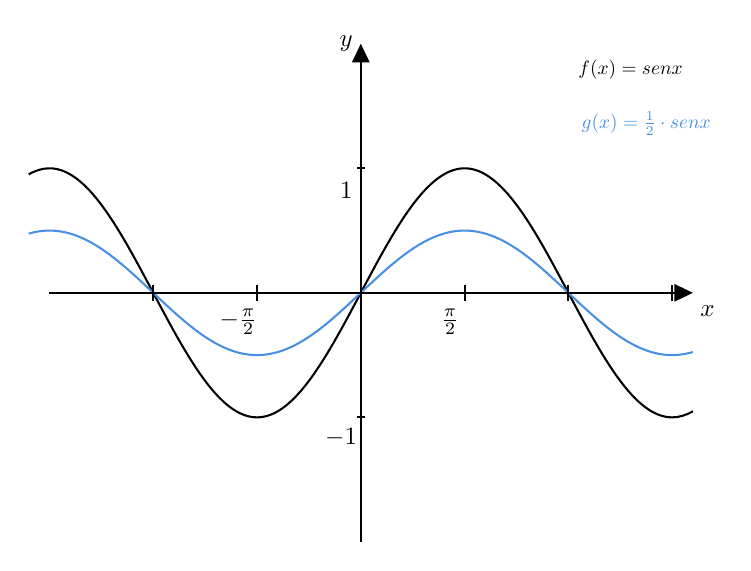
\begin{tikzpicture}[x=0.75pt,y=0.75pt,yscale=-1,xscale=1]
%uncomment if require: \path (0,300); %set diagram left start at 0, and has height of 300

%Shape: Wave [id:dp94416819522044] 
\draw   (180,102.94) .. controls (183.26,101.04) and (186.58,100) .. (190,100) .. controls (208.1,100) and (223.69,129.26) .. (240,160) .. controls (256.31,190.74) and (271.9,220) .. (290,220) .. controls (308.1,220) and (323.69,190.74) .. (340,160) .. controls (356.31,129.26) and (371.9,100) .. (390,100) .. controls (408.1,100) and (423.69,129.26) .. (440,160) .. controls (456.31,190.74) and (471.9,220) .. (490,220) .. controls (493.42,220) and (496.74,218.96) .. (500,217.06) ;
%Shape: Wave [id:dp05495114548578883] 
\draw  [color={rgb, 255:red, 74; green, 144; blue, 226 }  ,draw opacity=1 ] (180,131.47) .. controls (183.26,130.52) and (186.58,130) .. (190,130) .. controls (208.1,130) and (223.69,144.63) .. (240,160) .. controls (256.31,175.37) and (271.9,190) .. (290,190) .. controls (308.1,190) and (323.69,175.37) .. (340,160) .. controls (356.31,144.63) and (371.9,130) .. (390,130) .. controls (408.1,130) and (423.69,144.63) .. (440,160) .. controls (456.31,175.37) and (471.9,190) .. (490,190) .. controls (493.42,190) and (496.74,189.48) .. (500,188.53) ;
%Straight Lines [id:da13690129851328403] 
\draw    (190,160) -- (498,160) (240,156) -- (240,164)(290,156) -- (290,164)(340,156) -- (340,164)(390,156) -- (390,164)(440,156) -- (440,164)(490,156) -- (490,164) ;
\draw [shift={(500,160)}, rotate = 180] [fill={rgb, 255:red, 0; green, 0; blue, 0 }  ][line width=0.75]  [draw opacity=0] (8.93,-4.29) -- (0,0) -- (8.93,4.29) -- cycle    ;

%Straight Lines [id:da021329477973490496] 
\draw    (340,280) -- (340,42) (338,220) -- (342,220)(338,160) -- (342,160)(338,100) -- (342,100) ;
\draw [shift={(340,40)}, rotate = 450] [fill={rgb, 255:red, 0; green, 0; blue, 0 }  ][line width=0.75]  [draw opacity=0] (8.93,-4.29) -- (0,0) -- (8.93,4.29) -- cycle    ;


% Text Node
\draw (470,52.5) node [scale=0.7]  {$f( x) =senx$};
% Text Node
\draw (383,174) node [scale=0.9,color={rgb, 255:red, 0; green, 0; blue, 0 }  ,opacity=1 ]  {$\frac{\pi }{2}$};
% Text Node
\draw (281,174) node [scale=0.9,color={rgb, 255:red, 0; green, 0; blue, 0 }  ,opacity=1 ]  {$-\frac{\pi }{2}$};
% Text Node
\draw (333,110.5) node [scale=0.9]  {$1$};
% Text Node
\draw (330.5,229.5) node [scale=0.9]  {$-1$};
% Text Node
\draw (477.5,78.5) node [scale=0.7,color={rgb, 255:red, 74; green, 144; blue, 226 }  ,opacity=1 ]  {$g( x) =\frac{1}{2} \cdot senx$};
% Text Node
\draw (507,169) node [scale=0.9]  {$x$};
% Text Node
\draw (333,40) node [scale=0.9]  {$y$};


\end{tikzpicture}
